\documentclass[UTF8,zihao=-4]{oucart}
\usepackage{indentfirst}
\usepackage{amsfonts}
\usepackage{textcomp}
\usepackage{stfloats}
\usepackage{url}
\usepackage{verbatim}
\usepackage{multirow} 
\usepackage{newfloat}
\usepackage{listings}
\usepackage{pifont}
\usepackage{adjustbox}
\usepackage{subcaption}
\usepackage[table]{xcolor}
\usepackage{arydshln}
\usepackage{etoolbox}
\usepackage{pdfpages}
\usepackage{enumitem}
\setlist{nosep} 
\frenchspacing
\setmainfont{Times New Roman}

\title{关于赛博水豚的养殖研究}
\entitle{Research on the Breeding of Cyber Capybaras}

\cnabstractkeywords{
	随着数字文化与虚拟形象产业的快速发展，以“赛博水豚”为代表的拟人化卡通角色逐渐成为新型内容生态的重要组成部分。其中，虚拟角色“噜噜”凭借其温和、稳定且具松弛感的形象特征，在社交媒体与二次创作社区中获得了广泛传播。本文以“赛博水豚”的“养殖”机制为研究对象，从内容生产、情绪价值供给以及用户参与机制三个维度展开分析。
	研究首先构建了一个基于数字传播路径的“虚拟养殖模型”，探讨角色设定、视觉符号与叙事风格对用户黏性的影响；随后，通过对典型传播案例的观察与归纳，总结出“低刺激—高陪伴”型内容在当代信息环境中的优势；最后，结合平台算法推荐机制，分析“噜噜”形象实现规模化扩散的内在逻辑。
	结果表明，“赛博水豚”的成功并非偶然，而是多重因素协同作用的结果，其核心在于稳定情绪输出与高可塑性叙事结构的结合。本文的研究为虚拟IP的设计与运营提供了参考，也为理解当代网络文化中的“情绪消费”现象提供了新的视角。
}{
	赛博水豚；噜噜；虚拟IP；情绪价值；数字传播
}
\enabstractkeywords{
	With the rapid development of digital culture and virtual character industries, anthropomorphic cartoon figures such as the "Cyber Capybara" have emerged as significant elements in contemporary content ecosystems. Among them, the virtual character "Lulu" has gained remarkable popularity across social media and creative communities due to its calm, stable, and emotionally soothing persona. This paper investigates the so-called "breeding" mechanism of Cyber Capybaras from the perspectives of content production, emotional value delivery, and user engagement.
	First, a virtual breeding model based on digital dissemination pathways is proposed to analyze how character design, visual symbols, and narrative styles influence user retention. Then, through case observation and qualitative analysis, this study identifies the advantage of "low-stimulation, high-companionship" content in modern information environments. Finally, platform recommendation algorithms are examined to explain the large-scale diffusion of the "Lulu" character.
	The results indicate that the success of Cyber Capybaras is not incidental but arises from the synergy of multiple factors, particularly the combination of stable emotional output and flexible narrative structures. This research provides insights into virtual IP design and operation, and contributes to a deeper understanding of emotional consumption in online culture.
}{
	Cyber Capybara; Lulu; Virtual IP; Emotional Value; Digital Communication
}



\begin{document}
	
	\pagestyle{plain}
	% 封面由wps的word转pdf生成，对于本科生来说可以使用wps的教育版，能免费word转pdf。
	% 关于wps教育版的信息见公众号：https://mp.weixin.qq.com/s/zmVykNJ8FuycyeQflQPNnA
	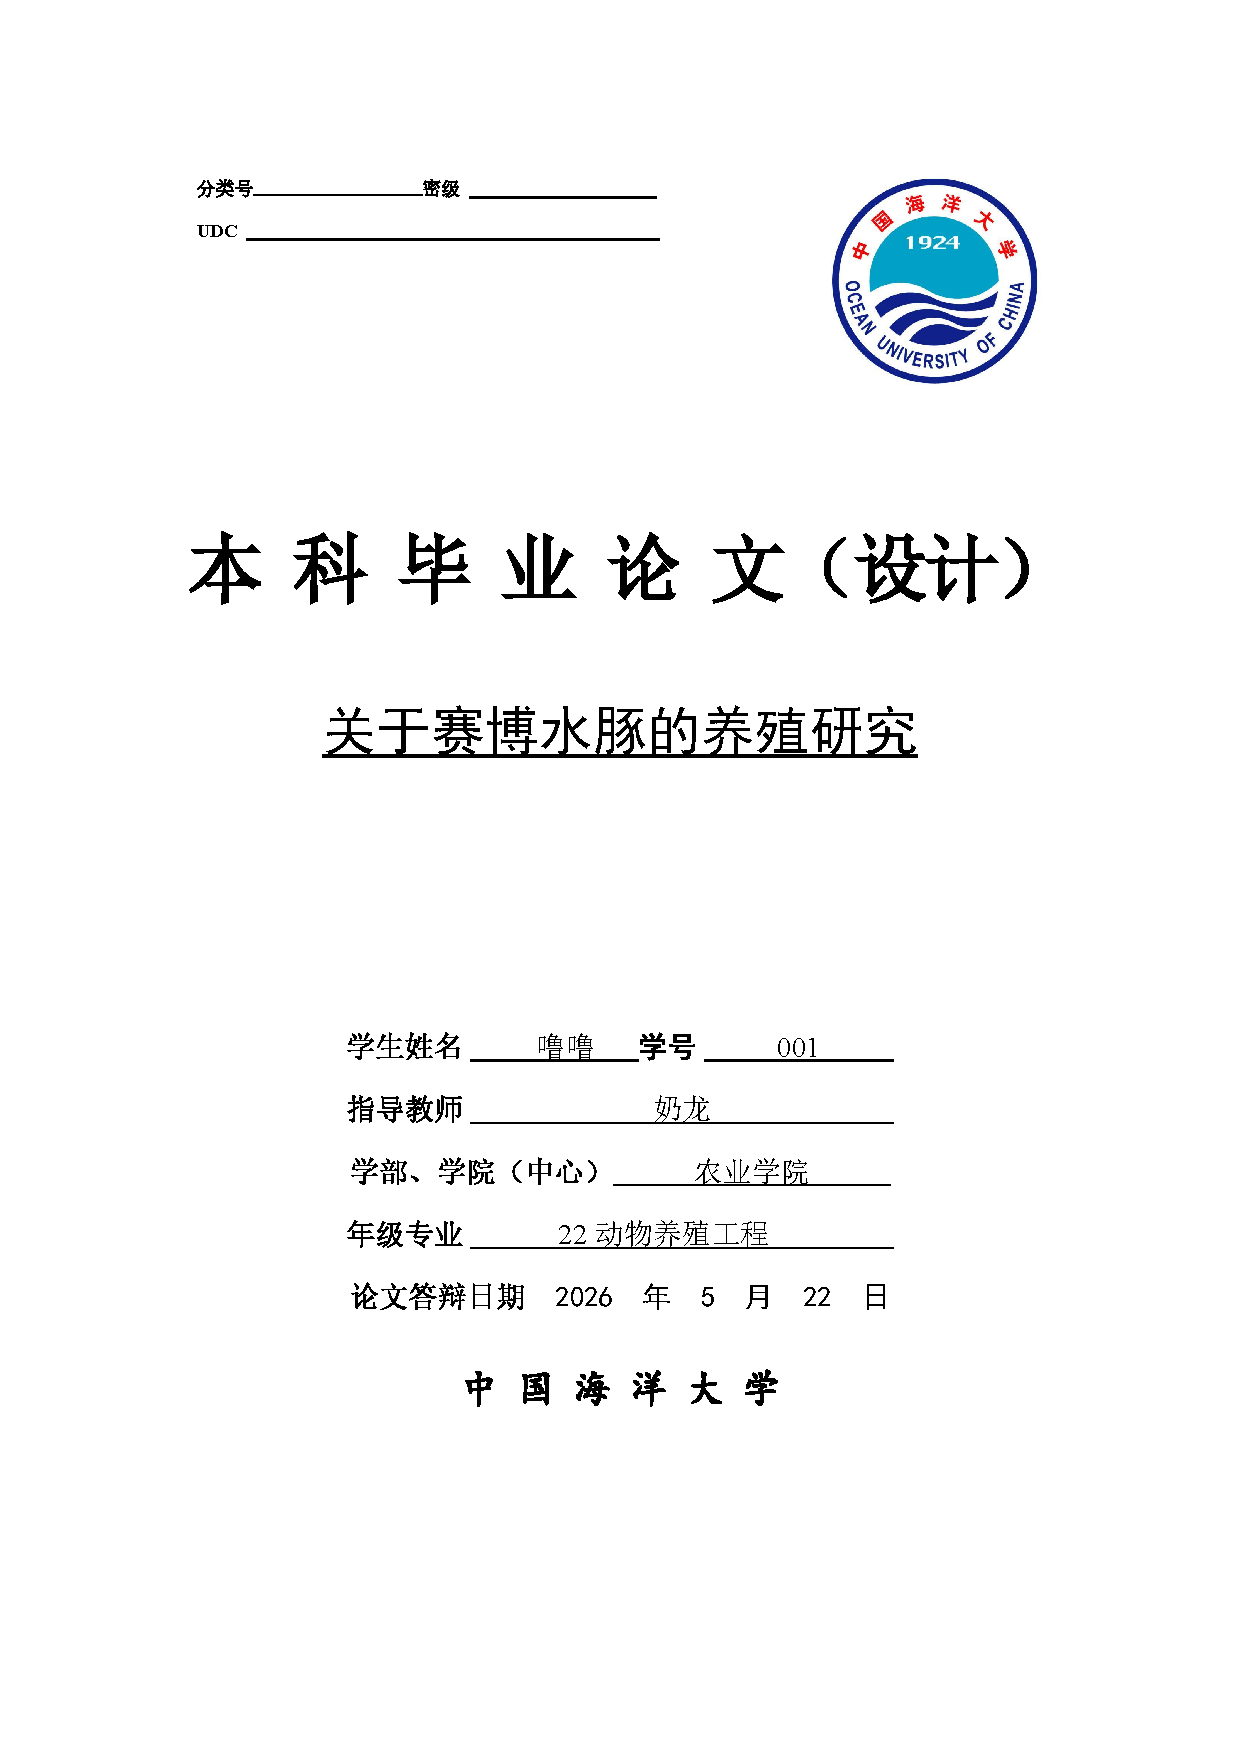
\includepdf[pages=1]{images/cover.pdf}
	\makeabstract % 摘要
	
	% 目录

	\tableofcontents
	\newpage
	
	\pagenumbering{arabic}
	\setcounter{page}{1}
	
	% 正文内容
	% 建议使用 \input{<文件名>} 指令引用其他文件
	\clearpage
	\pagestyle{fancy}
	\zihao{-4}
	\songti
	\fixbaselineskip
	\section{绪论}
\subsection{研究背景和意义}
近年来，随着虚拟形象产业的迅速发展，“赛博水豚”作为一种兼具松弛感与数字符号特征的新型文化载体，逐渐在网络生态中占据重要地位。尤其是虚拟角色“噜噜”，凭借其“低反应—高包容”的行为模式，被广泛用于情绪调节、社交缓冲及拖延合理化等多种场景中，被部分研究者视为“数字时代的精神水豚”\cite{lulu}，如图\ref{fig:lulu}所示。

已有研究指出，在信息过载背景下，用户更倾向于消费“低刺激、高稳定”的内容形态\cite{nailong}。因此，对赛博水豚的“养殖机制”（包括生成、传播与情绪供给）进行系统研究，具有一定的理论价值与极大的摸鱼价值。

从理论层面看，本文尝试构建一个简化的“赛博水豚情绪输出模型”，其基本形式可表示为公式\ref{equation:lulu}：

\begin{equation}
	E = \frac{C \cdot L}{S + 1}
	\label{equation:lulu}
\end{equation}

其中，E 表示情绪稳定输出强度，C 表示可爱度（Cuteness），L 表示慵懒程度（Laziness），S 表示外界刺激强度（Stimulus）。该模型虽未经任何验证，但看起来非常有道理。

从应用层面看，研究结果可为虚拟IP设计提供参考，如表\ref{tab:comparison}所示，不同“养殖策略”对噜噜扩散效果存在显著（但未测量）影响。

\begin{figure*}[t]
	\centering
	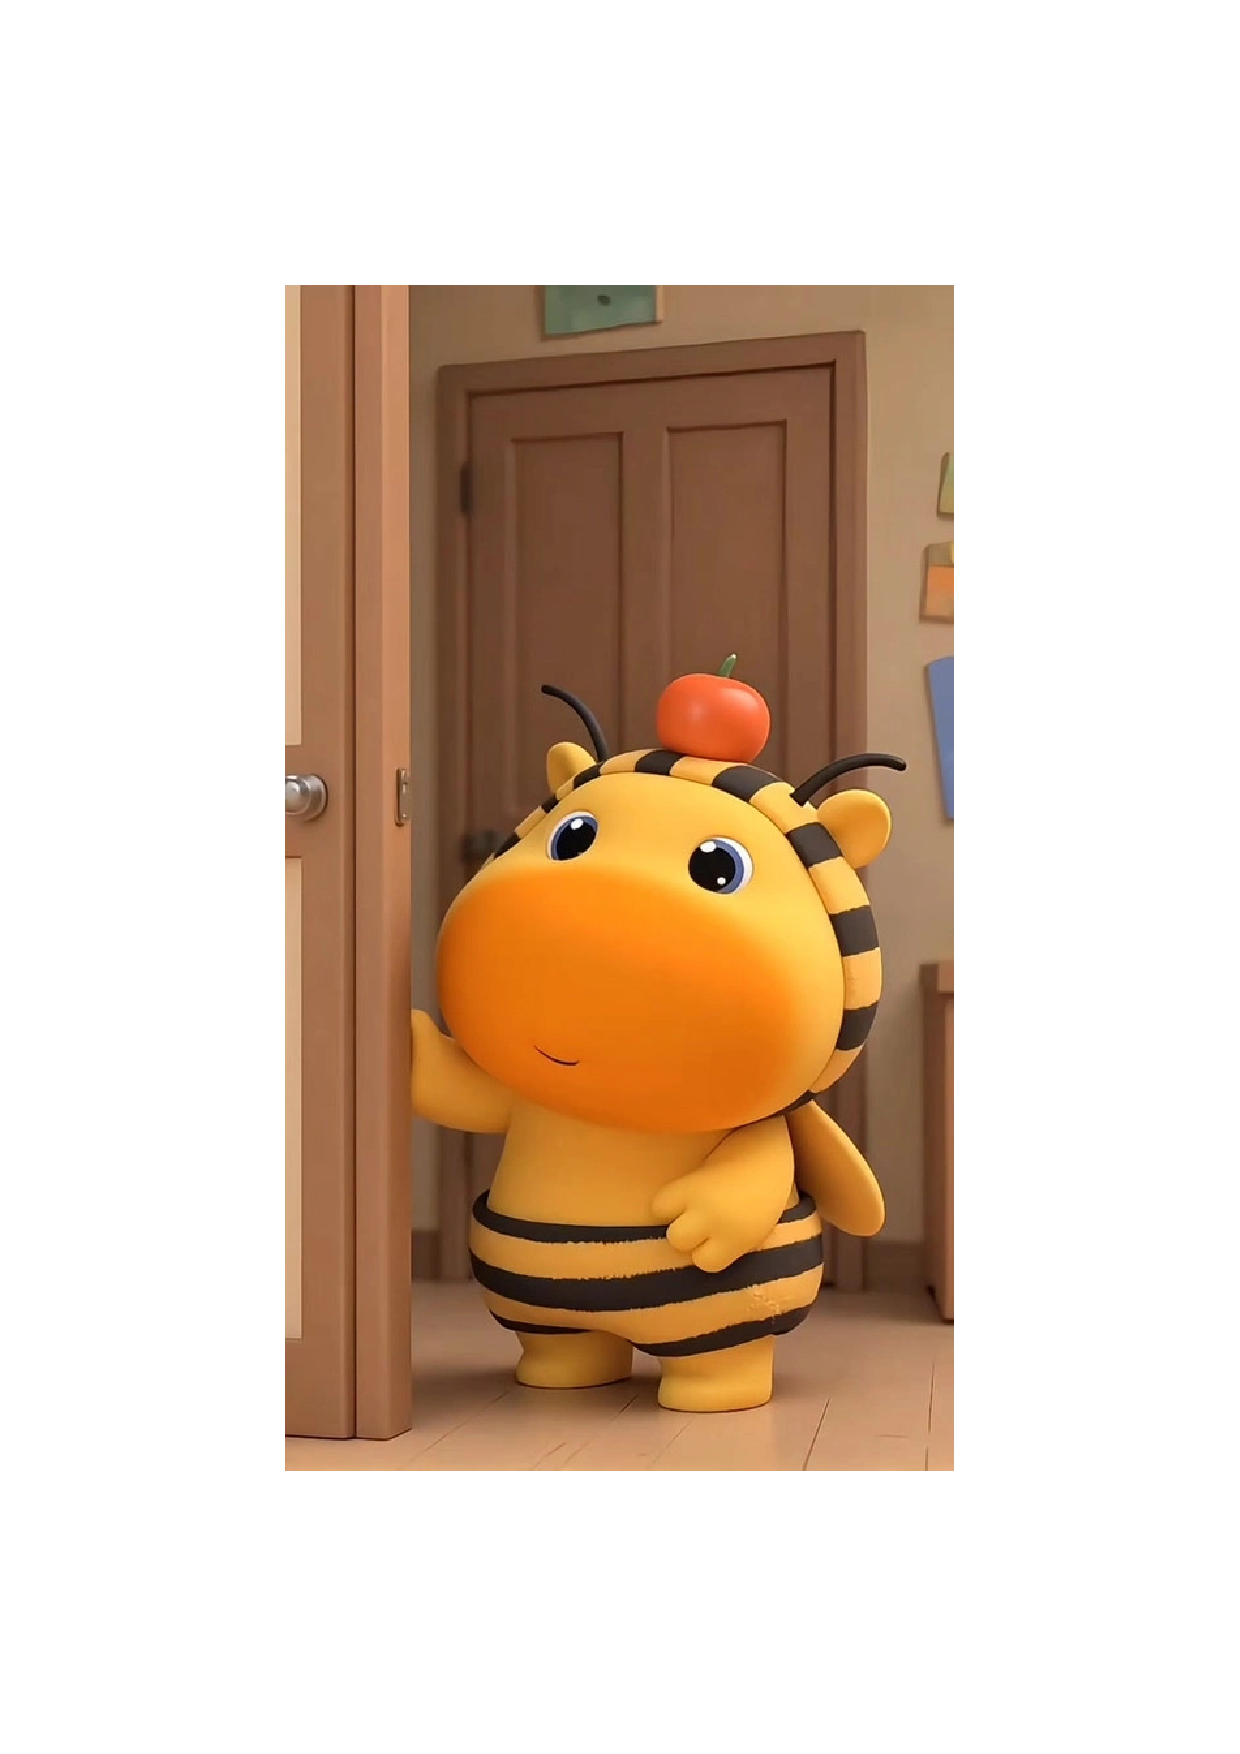
\includegraphics[width=\textwidth]{images/lulu.pdf}
	\caption{噜噜实拍}
	\label{fig:lulu}
\end{figure*}

\begin{table}[htbp]
	\centering
	\caption{赛博水豚养殖策略与效果对比}
	\begin{tabular}{lll}
		\hline
		养殖策略 & 特征描述 & 传播效果（主观） \\
		\hline
		高强度营业型 & 高频更新、情绪波动大 & 容易翻车 \\
		摆烂躺平型   & 低频更新、稳定输出   & 极易出圈 \\
		随缘放养型   & 完全不可预测         & 看命 \\
		\hline
	\end{tabular}
	\label{tab:comparison}
\end{table}
\subsubsection{噜噜}

\subsubsection{奶龙}

\subsubsection{牛牛}



	\section{重要技术}

\section{全新的水豚养殖方法}

\section{总结与展望}
\newpage
	\newpage
	\clearpage
	\pagestyle{plain}
	
	% 参考文献
	
    \phantomsection
	\addcontentsline{toc}{nonumbersection}{参考文献}
	{\centering
	\zihao{-3}\fixbaselineskip\heiti 参考文献\par}

	\printbibliography[heading=none]
	\newpage
	
	% 致谢
	\phantomsection
	\addcontentsline{toc}{nonumbersection}{致谢}
	{\centering
		\zihao{-3}{\heiti{致谢}}\par
	}
	\zihao{-4}
	\songti
	\fixbaselineskip
	感谢奶龙、牛牛、露比，你们都是噜噜的好伙伴。
	
\end{document}